\section{SG\_\-File\_\-TXT Class Reference}
\label{class_s_g___file___t_x_t}\index{SG_File_TXT@{SG\_\-File\_\-TXT}}
This is a file writer for the solar system description.  


{\tt \#include $<$SG\_\-File\_\-TXT.h$>$}

Inheritance diagram for SG\_\-File\_\-TXT::\begin{figure}[H]
\begin{center}
\leavevmode
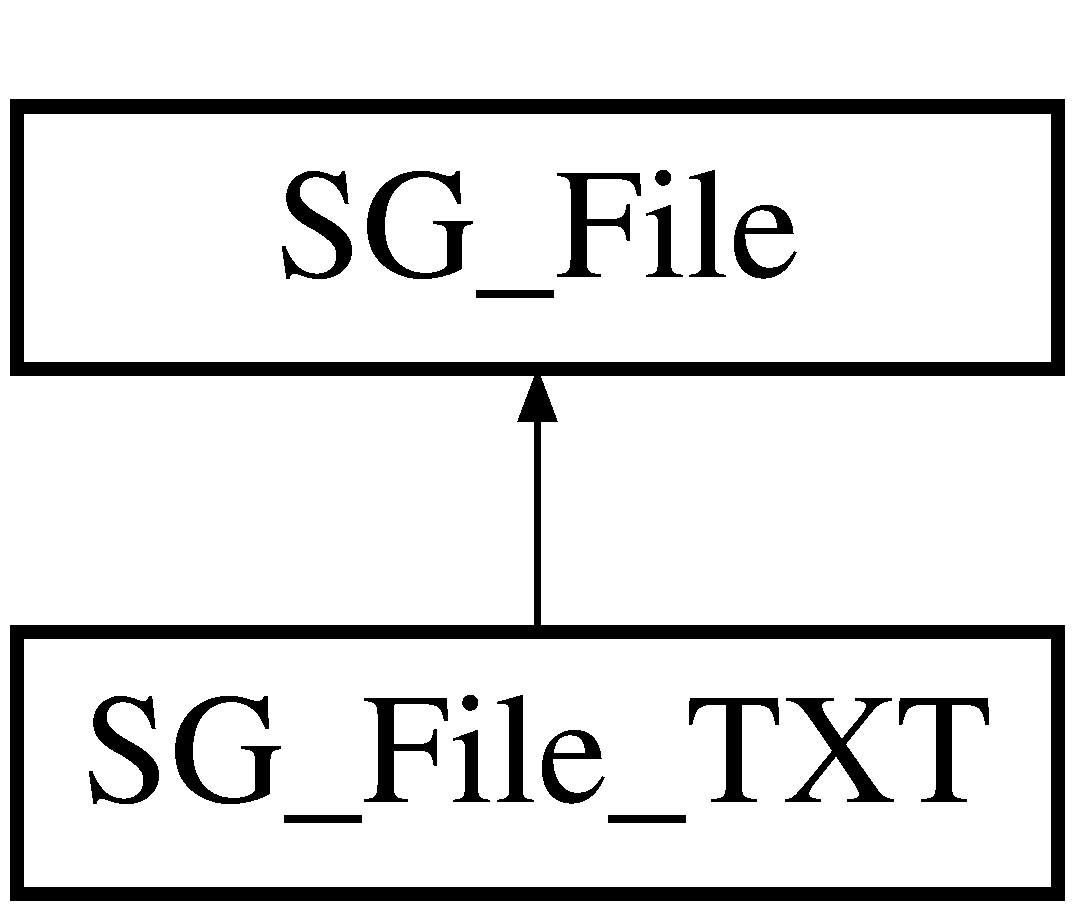
\includegraphics[height=2cm]{class_s_g___file___t_x_t}
\end{center}
\end{figure}
\subsection*{Public Member Functions}
\begin{CompactItemize}
\item 
{\bf SG\_\-File\_\-TXT} (SG\_\-String filename, long seed)\label{class_s_g___file___t_x_t_a0}

\begin{CompactList}\small\item\em Constructor. \item\end{CompactList}\item 
{\bf $\sim$SG\_\-File\_\-TXT} ()\label{class_s_g___file___t_x_t_a1}

\begin{CompactList}\small\item\em Destructor. \item\end{CompactList}\end{CompactItemize}
\subsection*{Protected Member Functions}
\begin{CompactItemize}
\item 
void {\bf add\-Value} (SG\_\-String name, bool value)\label{class_s_g___file___t_x_t_b0}

\begin{CompactList}\small\item\em Write a data in the file. \item\end{CompactList}\item 
void {\bf add\-Value} (SG\_\-String name, char $\ast$value, SG\_\-String comment)\label{class_s_g___file___t_x_t_b1}

\begin{CompactList}\small\item\em Write a data in the file. \item\end{CompactList}\item 
void {\bf add\-Value} (SG\_\-String name, SG\_\-String value, SG\_\-String comment)\label{class_s_g___file___t_x_t_b2}

\begin{CompactList}\small\item\em Write a data in the file. \item\end{CompactList}\item 
void {\bf add\-Value} (SG\_\-String name, long double value, SG\_\-String comment)\label{class_s_g___file___t_x_t_b3}

\begin{CompactList}\small\item\em Write a data in the file. \item\end{CompactList}\item 
void {\bf add\-Int\-Value} (SG\_\-String name, long double value, SG\_\-String comment)\label{class_s_g___file___t_x_t_b4}

\begin{CompactList}\small\item\em Write a data in the file (converted to integer). \item\end{CompactList}\item 
void {\bf add\-Percentage} (SG\_\-String name, long double value)\label{class_s_g___file___t_x_t_b5}

\begin{CompactList}\small\item\em Write a data in the file. \item\end{CompactList}\item 
void {\bf add\-Section} (SG\_\-String name)\label{class_s_g___file___t_x_t_b6}

\begin{CompactList}\small\item\em Add a section header in the file. \item\end{CompactList}\item 
void {\bf close\-Section} (SG\_\-String name)\label{class_s_g___file___t_x_t_b7}

\begin{CompactList}\small\item\em Add a section ender in the file. \item\end{CompactList}\item 
void {\bf sub\-Section} ()\label{class_s_g___file___t_x_t_b8}

\begin{CompactList}\small\item\em Add a sub-section in the file. \item\end{CompactList}\item 
void {\bf add\-Line} ()\label{class_s_g___file___t_x_t_b9}

\begin{CompactList}\small\item\em Add a separator line in the file. \item\end{CompactList}\end{CompactItemize}


\subsection{Detailed Description}
This is a file writer for the solar system description. 

The output format is an explicit plain text file. 



The documentation for this class was generated from the following files:\begin{CompactItemize}
\item 
E:/sphinx/LFE/lib\_\-stargen/SG\_\-File\_\-TXT.h\item 
E:/sphinx/LFE/lib\_\-stargen/SG\_\-File\_\-TXT.cpp\end{CompactItemize}
